  \section{Symulacje Numeryczne}
  
  (SZCZEGÓŁY TECHNICZNE / LICZBOWE?)
  
  
  \subsection{Oprogramowanie}

  Do oprogramowania symulacji wybrałem język Java, jako oferujący dobrą wydajność w obliczeniach numerycznych, z dojrzałym ekosystemem narzędzi i bibliotek oraz wieloplatformowy. Oskryptowanie zestawów symulacji (''przemiatanie'' po parametrach, wiele powtórzeń dla uśrednienia wyników) napisałem w języku Groovy.
  
  Kod źródłowy jest dostępny jako open-source i dostępny w serwisie GitHub pod adresem http://github.com/tomash/zzzzz

  \subsubsection{Obliczanie Widma Mocy}

  \begin{equation}
    |P| = F(x)^2
  \end{equation}

  \subsubsection{Obliczanie Signal-to-Noise Ratio}

  Stosunek sygnał-szum obliczałem poprzez podzielenie wartości lokalnie najwyższej (tj. piku głównego) przez sumę 10 wartości sąsiadujących (5 niższych, 5 wyższych).
  
  \subsection{Pojedynczy Neuron}
  
  Przed przystąpieniem do rozwiązywania układów wieloneuronowych rozpocząłem symulacje od zbadania pojedynczego neuronu, jak opisywany w pracy A. Longtin \cite{longtin}. Dzięki temu mogłem sprawdzić zarówno poprawność własnego oprogramowania, jak i model oraz zestaw parametrów opisane w wyżej wymienionej publikacji.
  
  Stochastyczne równania różniczkowe składające się na szum Ornsteina-Uhlenbecka całkowałem według metody opisanej w pracy Mannella, Palleschi \cite{mannella}. Po rozwiązaniu przedstawionego tam równania, przyrost szumu $\eta (t)$ liczony był następująco:

  \begin{equation} \label{eq:deta}
    d\eta(t) = dt(\lambda \xi_1(t) - \lambda \eta(t)) + \lambda \xi_2(t) \sqrt{dt}
  \end{equation}

  Gdzie $\xi_n(t)$ to szum gaussowski w chwili t.
  
  Przebieg czasowy potencjału pojedynczego neuronu, z zestawem parametrów jak w \cite{longtin}.
  
  \begin{figure}
    \begin{center}
      \begin{tabular}{cc}
        \resizebox{100mm}{!}{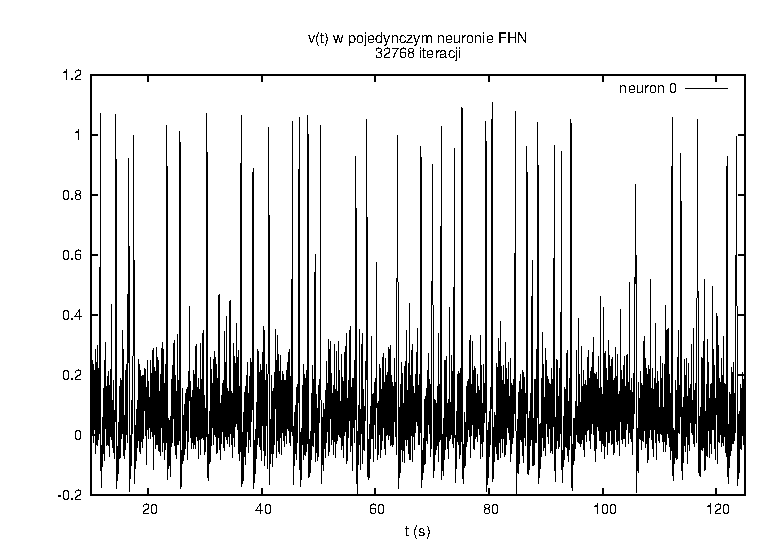
\includegraphics[width=140mm]{images/1neuron/1}} \\
        \resizebox{100mm}{!}{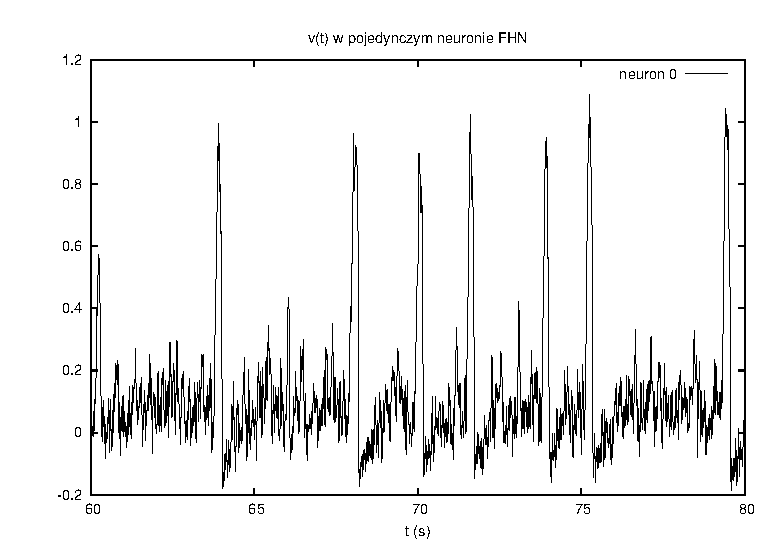
\includegraphics[width=140mm]{images/1neuron/2}} \\
      \end{tabular}
      \caption{Odtworzenie wyników Longtina. 32768 kroków iteracji, $\Delta t = 1/256 s$ (łączny czas symulacji 128s), $t_c=0.01$, $q=1.0$, $\epsilon = 0.005$, $D=1E{-5}$}
      \label{sym1v}
    \end{center}
  \end{figure}

  Jest to przebieg zgodny z zaobserwowanym w pracy A. Longtin.

  \begin{figure}
    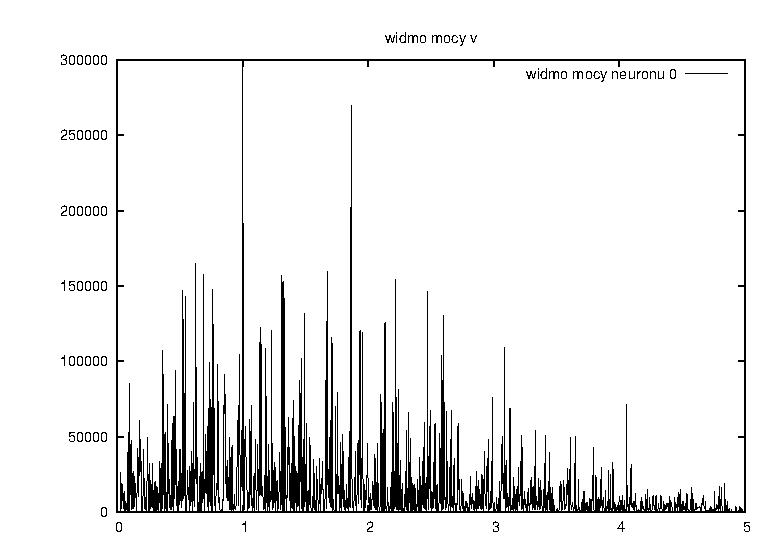
\includegraphics[width=140mm]{images/1neuron/3}
    \caption{FFT odtworzenie wyników longtina}
    \label{sym1fft}
  \end{figure}

  
  \subsection{Układy Neuronów Bez Opóźnienia}
  
  Następnym krokiem pracy było połączenie neuronów (początkowo dwóch) w ''sznur'', z sygnałem przekazywanym w jedną stronę, tzn. sygnał z neuronu i jest odbierany przez neuron i-1 (neuron o numerze 0 nie przekazuje swojego sygnału dalej). Neurony w układzie działały według równania zaproponowanego w rozdziale ~\ref{sec:przesuniecie_fazy}, bez opóźnienia (czyli $\tau_{n} = 0$).

  Ważnym elementem tego etapu badań było dobranie nowej wartości skalowania szumu D. Dotychczasowa wartość, czyli 1E-5, powodowała maksymalizację SNR w pojedynczym neuronie, ale w macierzach neuronów powoduje tłumienie wpływu sygnałów odebranych od połączonych neuronów (przesterowanie).

  Po wielu symulacjach z różnymi zakresami parametrów (patrz też wykres \ref{fig:graphics:snr_c_d_3d}) ustaliłem wartość D w okolicach $D=5E{-6}$ jako pozwalającą zaobserwować SR w pojedynczym neuronie jak i obserwować wyraźne zwiększanie SNR w wyniku odbierania sygnału od połączonych neuronów. Dla potwierdzenia tej hipotezy dalsze symulacje prowadzone były dla wartości D w zakresie od $D=1E{-6}$ do $D=2E{-5}$. Ważna jest też czułość na sygnał odebrany od połączonego neuronu, ustaliłem ją na poziomie 0.03 (czterokrotnie niższym niż skalowanie sygnału periodycznego).

  \begin{figure}
    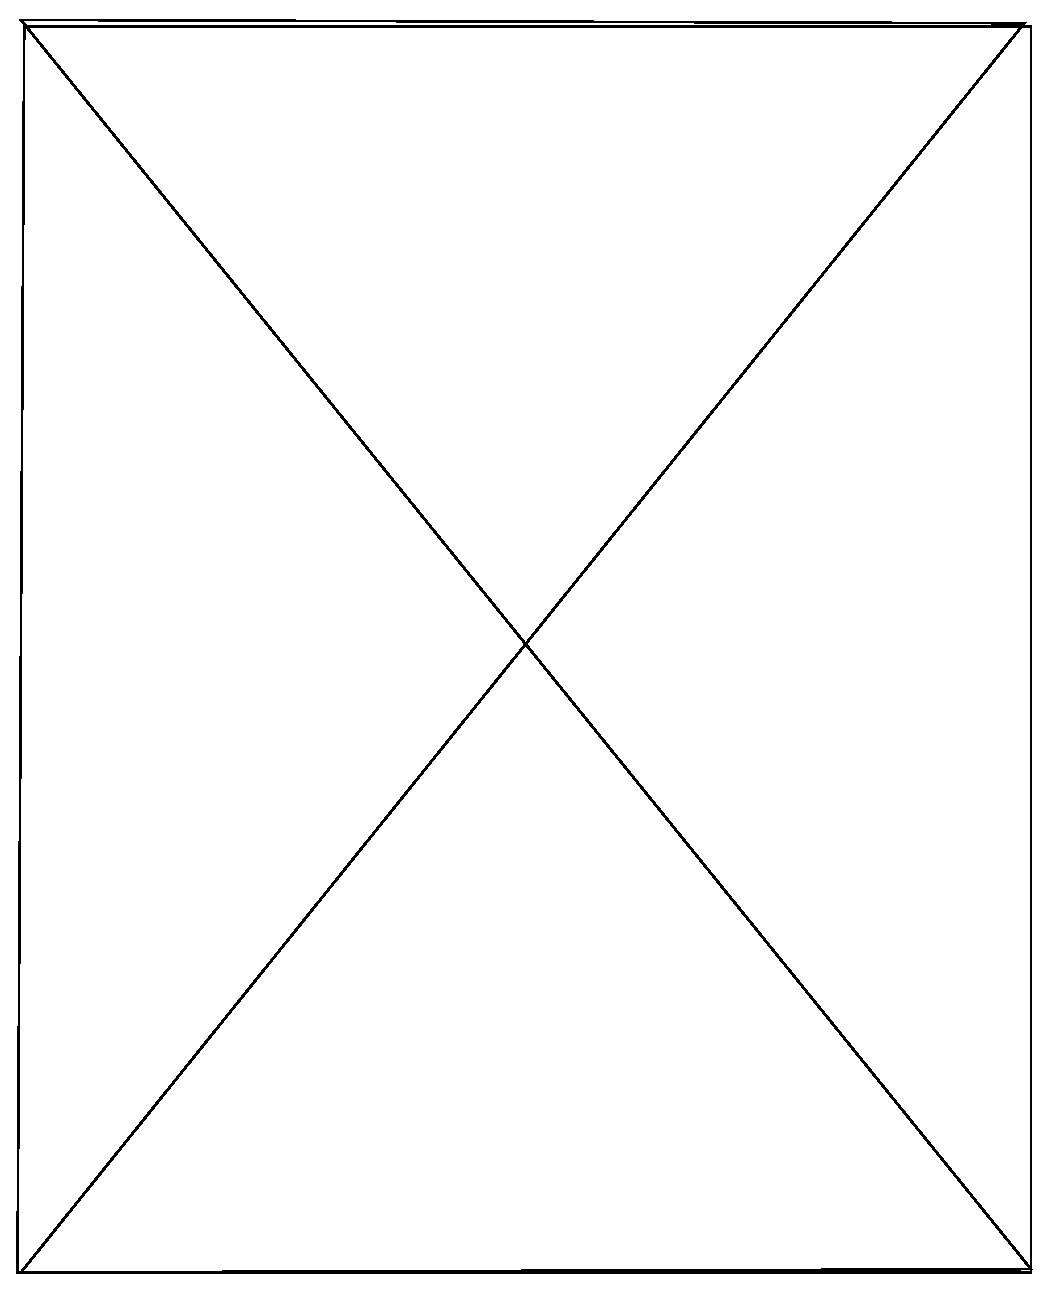
\includegraphics[width=120mm]{images/pending}
    \caption{Układ kilku (?) neuronów bez opóźnienia. Widać wyraźny wzrost SNR zgodnie z ''kierunkiem'' przekazywania sygnału. SNR liczony na podstawie nienormalizowanego widma mocy. 262144 ($2^{18}$) kroków iteracji dla każdego zestawu parametrów.}
    \label{fig:graphics:sim:x}
  \end{figure}

  Zaobserwowane przebiegi czasowe były zgodne ze spodziewanym analitycznie wynikiem: z każdym kolejnym neuronem w łańcuchu następował wzrost SNR (do wartości granicznej około 2000) ze względu na wzrost prawdopodobieństwa wzbudzenia w przypadku wzbudzenia neuronu sąsiedniego.

  \begin{figure}
    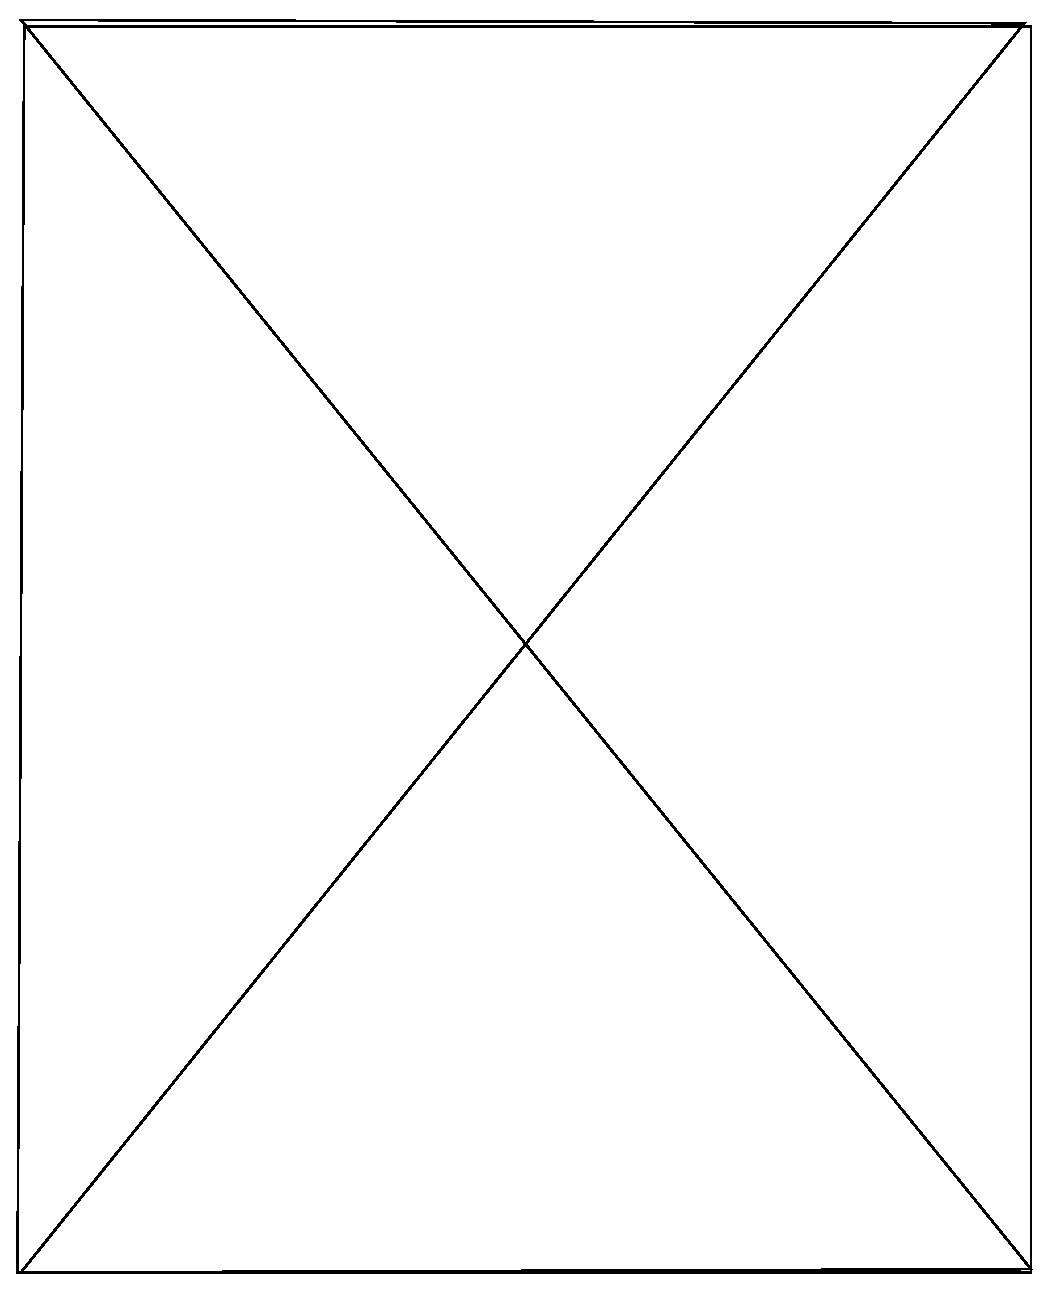
\includegraphics[width=120mm]{images/pending}
    \caption{Układ kilku 9 neuronów rozciągły przestrzennie o przesunięciu fazowym $\phi_i = 0.111 T i, \Delta \phi = 0.111 T$ i z opóźnieniem transmisji dobranym do kompensowania rozciągłości przestrzennej $c = \Delta \phi$. Wzrost SNR zgodnie z ''kierunkiem'' przekazywania sygnału jest maksymalny, do wartości granicznej około 1600. SNR liczony na podstawie nienormalizowanego widma mocy. 262144 ($2^{18}$) kroków iteracji dla każdego zestawu parametrów.}
    \label{fig:graphics:sim:2010_10_03}
  \end{figure}

  Na rysunku \ref{fig:graphics:sim:2010_10_03} można zaobserwować ciekawe i wymagające dalszych badań zjawisko. Otóż po osiągnięciu przez neuron i-ty regularności bliskiej maksymalnej ($SNR \approx 1500$), w neuronie i-1, do którego przekazywany jest sygnał, następował wyraźny spadek SNR. Wynika z tego, że zbyt periodyczny sygnał wejściowy przesterowuje neuron i tym samym wywołuje suboptymalny SR.

  
  \subsection{Układy Neuronów Z Opóźnieniem}
  
  Do układu opisanego powyżej dodałem opóźnienie w przekazywaniu sygnałów, w sposób opisany w rozdziale ~\ref{sec:przesuniecie_fazy}

  
  \subsubsection{Macierz Dwóch Neuronów}

  Pierwszym krokiem w badaniu macierzy neuronów z opóźnieniem uczyniłem zbadanie macierzy dwuelementowej, celem znalezienia zależności pomiędzy podstawowymi parametrami symulacji.

  Przez c oznaczyłem opóźnienie transmisji, jako wielokrotność okresu sygnału periodycznego. Przesunięcie fazowe sygnału periodycznego p wynosiło pół okresu.
  Znaleziona zależność SNR (WYKRES) od c oraz D (skalowanie szumu) posiada bardzo wyraźną ''grań'' dla c=0.5, co potwierdza oczekiwania: maksymalizację SNR można osiągnąć poprzez kompensację przesunięcia fazowego (rozciągłości przestrzennej) identycznym (lub prawie identycznym) opóźnieniem w transmisji.

  \begin{figure}
    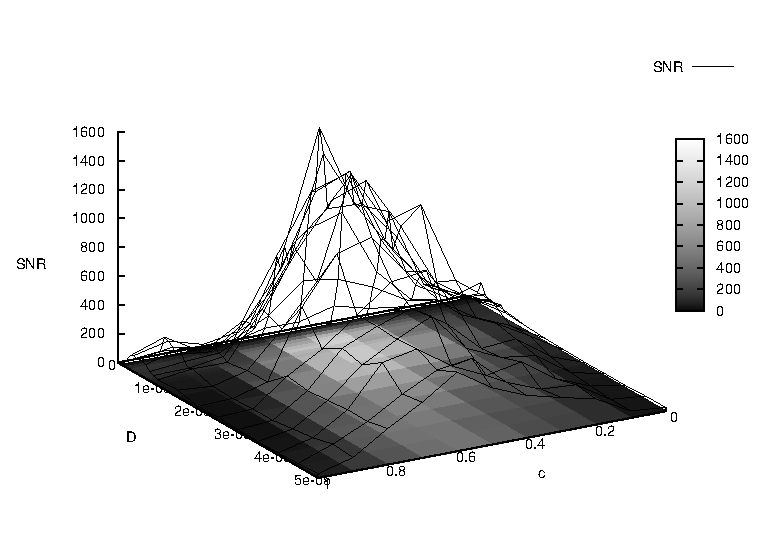
\includegraphics[width=140mm]{images/2neuron/3d}
    \caption{Dwa neurony, SNR w ''odbierającym'' w zależności od opóźnienia w transmisji c (jako wielokrotność T), dla przesunięcia fazowego równego 0.5T. Widać wyraźną ''grań'' kiedy c = p (= 0.5T)}
    \label{fig:graphics:snr_c_d_3d}
  \end{figure}

  Wyniki dla dwóch neuronów potwierdzają hipotezę. Jednakże dla analizy relacji skalowania symulowana była także macierz 9 neuronów z opóźnieniem transmisji.

  \subsubsection{Macierz 9 Neuronów Z Opóźnieniem}

  Pierwszym krokiem było zbadanie macierzy neuronów FHN połączonych tak, aby opóźnienie transmisji kompensowało rozciągłość przestrzenną, czyli $c = \Delta \phi$. Zbudowanie

  \begin{figure}
    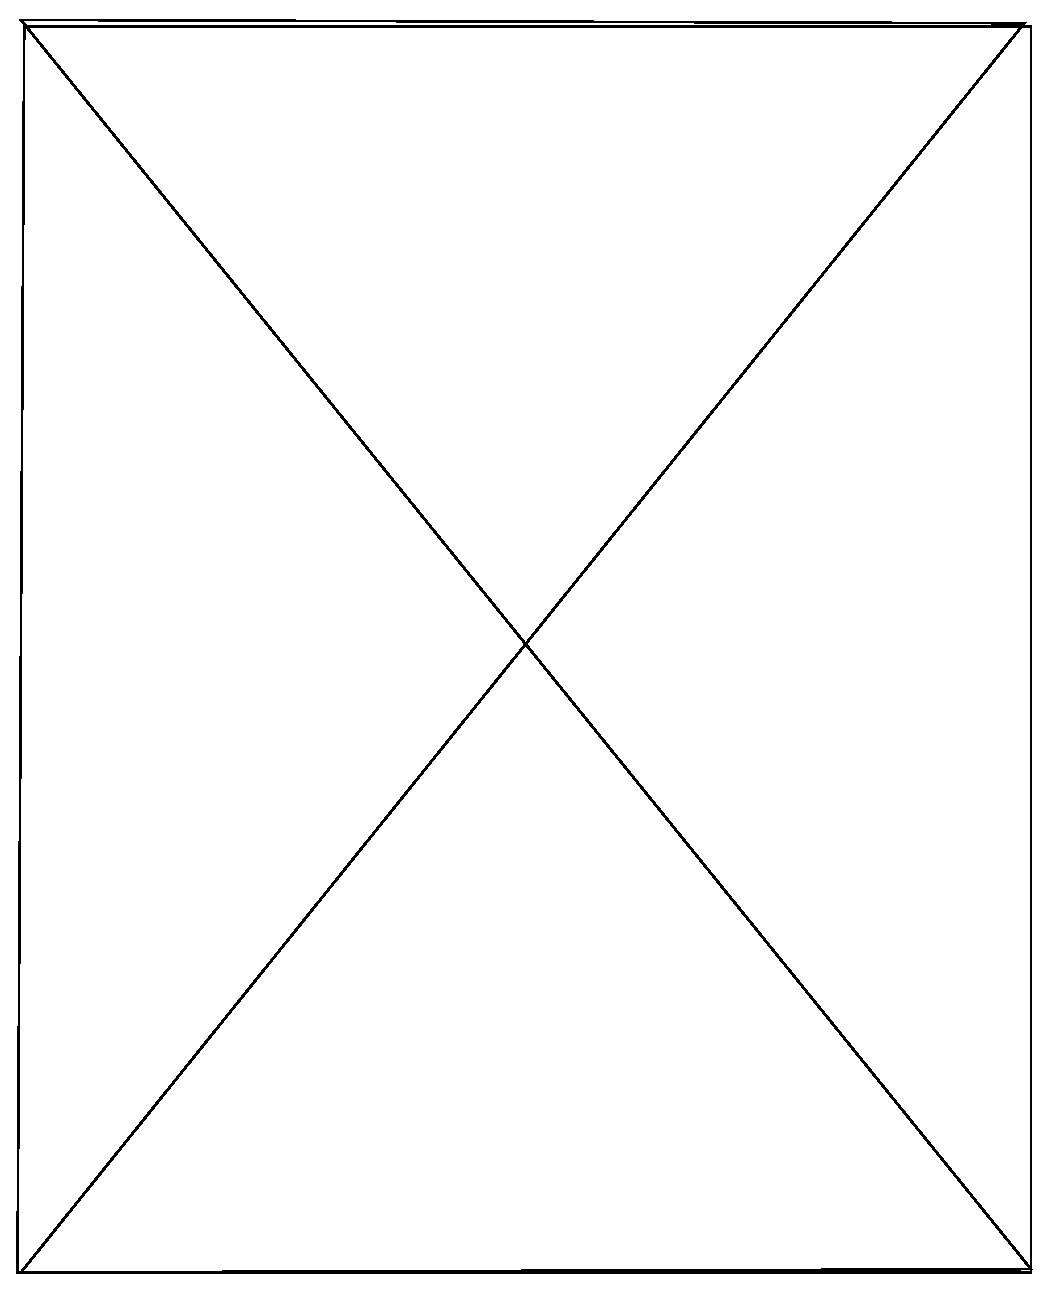
\includegraphics[width=120mm]{images/pending}
    \caption{Układ kilku 9 neuronów rozciągły przestrzennie o przesunięciu fazowym $\phi_i = 0.111 T i, \Delta \phi = 0.111 T$ i z opóźnieniem transmisji dobranym do kompensowania rozciągłości przestrzennej $c = \Delta \phi$. Wzrost SNR zgodnie z ''kierunkiem'' przekazywania sygnału jest maksymalny, do wartości granicznej około 1600. SNR liczony na podstawie nienormalizowanego widma mocy. 262144 ($2^{18}$) kroków iteracji dla każdego zestawu parametrów.}
    \label{fig:graphics:sim:2010_10_03b}
  \end{figure}

  Na rysunku \ref{fig:graphics:sim:2010_10_03} można zaobserwować 

  ciekawe i wymagające dalszych badań zjawisko. Otóż po osiągnięciu przez neuron i-ty maksymalnej regularności ($SNR \approx 1500$), w neuronie i-1, do którego przekazywany jest sygnał, następuje wyraźny spadek SNR. Wynika z tego, że zbyt periodyczny sygnał wejściowy przesterowuje neuron i wykracza poza zakres optymalności SR.
  

